

\tikzset{every picture/.style={line width=0.75pt}} %set default line width to 0.75pt        

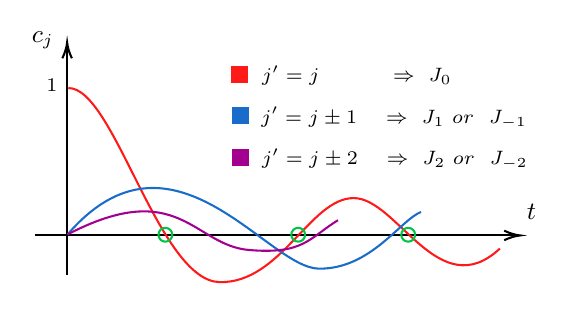
\begin{tikzpicture}[x=0.75pt,y=0.75pt,yscale=-1,xscale=1]
%uncomment if require: \path (0,130); %set diagram left start at 0, and has height of 130

%Straight Lines [id:da42292147954355674] 
\draw    (23,121) -- (23,11) ;
\draw [shift={(23,9)}, rotate = 90] [color={rgb, 255:red, 0; green, 0; blue, 0 }  ][line width=0.75]    (7.65,-2.3) .. controls (4.86,-0.97) and (2.31,-0.21) .. (0,0) .. controls (2.31,0.21) and (4.86,0.98) .. (7.65,2.3)   ;
%Straight Lines [id:da0938116227302922] 
\draw    (7.5,102) -- (239.25,102) ;
\draw [shift={(241.25,102)}, rotate = 180] [color={rgb, 255:red, 0; green, 0; blue, 0 }  ][line width=0.75]    (7.65,-2.3) .. controls (4.86,-0.97) and (2.31,-0.21) .. (0,0) .. controls (2.31,0.21) and (4.86,0.98) .. (7.65,2.3)   ;
%Curve Lines [id:da7388142079293656] 
\draw [color={rgb, 255:red, 255; green, 26; blue, 26 }  ,draw opacity=1 ]   (23.58,31) .. controls (45.58,30.5) and (67.08,124) .. (96.58,124.5) .. controls (126.08,125) and (140.08,84) .. (161.08,84) .. controls (182.08,84) and (202,135.83) .. (231.5,108.33) ;
%Curve Lines [id:da2797400644106053] 
\draw [color={rgb, 255:red, 25; green, 108; blue, 201 }  ,draw opacity=1 ]   (23.25,101.5) .. controls (73.75,43) and (119.33,117.67) .. (144.25,118) .. controls (169.17,118.33) and (183.5,94.67) .. (193.5,90.67) ;
%Curve Lines [id:da34662757016201506] 
\draw [color={rgb, 255:red, 163; green, 0; blue, 143 }  ,draw opacity=1 ]   (23.25,101.5) .. controls (76.83,73.67) and (83.83,106.67) .. (110.5,109) .. controls (137.17,111.33) and (139.83,103) .. (153.5,94.67) ;
%Shape: Circle [id:dp028498302535310938] 
\draw  [color={rgb, 255:red, 0; green, 196; blue, 69 }  ,draw opacity=1 ][line width=0.75]  (67,101.67) .. controls (67,99.83) and (68.49,98.33) .. (70.33,98.33) .. controls (72.17,98.33) and (73.67,99.83) .. (73.67,101.67) .. controls (73.67,103.51) and (72.17,105) .. (70.33,105) .. controls (68.49,105) and (67,103.51) .. (67,101.67) -- cycle ;
%Shape: Circle [id:dp30028872852521227] 
\draw  [color={rgb, 255:red, 0; green, 196; blue, 69 }  ,draw opacity=1 ][line width=0.75]  (131,101.67) .. controls (131,99.83) and (132.49,98.33) .. (134.33,98.33) .. controls (136.17,98.33) and (137.67,99.83) .. (137.67,101.67) .. controls (137.67,103.51) and (136.17,105) .. (134.33,105) .. controls (132.49,105) and (131,103.51) .. (131,101.67) -- cycle ;
%Shape: Circle [id:dp6051192164240733] 
\draw  [color={rgb, 255:red, 0; green, 196; blue, 69 }  ,draw opacity=1 ][line width=0.75]  (184,101.67) .. controls (184,99.83) and (185.49,98.33) .. (187.33,98.33) .. controls (189.17,98.33) and (190.67,99.83) .. (190.67,101.67) .. controls (190.67,103.51) and (189.17,105) .. (187.33,105) .. controls (185.49,105) and (184,103.51) .. (184,101.67) -- cycle ;
%Shape: Square [id:dp9109798777185496] 
\draw  [draw opacity=0][fill={rgb, 255:red, 255; green, 26; blue, 26 }  ,fill opacity=1 ] (102,20.33) -- (110.17,20.33) -- (110.17,28.5) -- (102,28.5) -- cycle ;
%Shape: Square [id:dp708254493093753] 
\draw  [draw opacity=0][fill={rgb, 255:red, 25; green, 108; blue, 201 }  ,fill opacity=1 ] (102.33,40.33) -- (110.5,40.33) -- (110.5,48.5) -- (102.33,48.5) -- cycle ;
%Shape: Square [id:dp732226894539835] 
\draw  [draw opacity=0][fill={rgb, 255:red, 163; green, 0; blue, 143 }  ,fill opacity=1 ] (102.67,60.33) -- (110.83,60.33) -- (110.83,68.5) -- (102.67,68.5) -- cycle ;

% Text Node
\draw (4.5,2.4) node [anchor=north west][inner sep=0.75pt]  [font=\small]  {$c_{j}$};
% Text Node
\draw (11.5,24.9) node [anchor=north west][inner sep=0.75pt]  [font=\scriptsize]  {$1$};
% Text Node
\draw (115.33,18.73) node [anchor=north west][inner sep=0.75pt]  [font=\scriptsize]  {$j'=j\ \ \ \ \ \ \ \ \ \Rightarrow \ J_{0}$};
% Text Node
\draw (115,38.73) node [anchor=north west][inner sep=0.75pt]  [font=\scriptsize]  {$j'=j\pm 1\ \ \ \Rightarrow \ J_{1} \ \text{or} \ \ J_{-1}$};
% Text Node
\draw (115.33,58.73) node [anchor=north west][inner sep=0.75pt]  [font=\scriptsize]  {$j'=j\pm 2\ \ \ \Rightarrow \ J_{2} \ \text{or} \ \ J_{-2}$};
% Text Node
\draw (243,85.4) node [anchor=north west][inner sep=0.75pt]  [font=\small]  {$t$};


\end{tikzpicture}
